\section{Übertragungsverfahren}
Das zu übertragende Signal ist ein analoges Messignal mit Netzfrequenz, welches von der Hochspannungsanlage stammt. Die Amplitude wird durch den Eingangswiderstand der Sendeeinheit bestimmt. Die zur Verfügung stehenden Dioden können analoge sowie digitale Signale übertragen. Aufgrund dessen stehen mehrere Übertragungsverfahren zur Auswahl.
In diesem Kapitel werden einige in Frage kommenden Übertragungsverfahren vorgestellt und evaluiert.
\subsection{Analoge Übertragungsarten}
\subsubsection{Direkte Übertragung}
Eine Möglichkeit das Signal zu übertragen ist, dieses nach Aufbereitung direkt auf die Dioden zu geben.
Durch diese Anordnung ist jedoch nicht garantiert, dass das Messignal bei variierender Länge des Lichtwellenleiters mit gleicher Amplitude rekonsturiert werden kann. Die Dämpfung des Lichtwellenleiters erfordert eine Kalibration auf verschiedene Längen der Übertragungs\-strecke.
\subsubsection{Frequenzmodulation}
\begin{figure}[H]
\centering
  \scalebox{0.7}{\begin{large}$% Title: glps_renderer figure
% Creator: GL2PS 1.3.8, (C) 1999-2012 C. Geuzaine
% For: Octave
% CreationDate: Fri Oct 21 17:46:43 2016
\setlength{\unitlength}{1pt}
\begin{picture}(0,0)
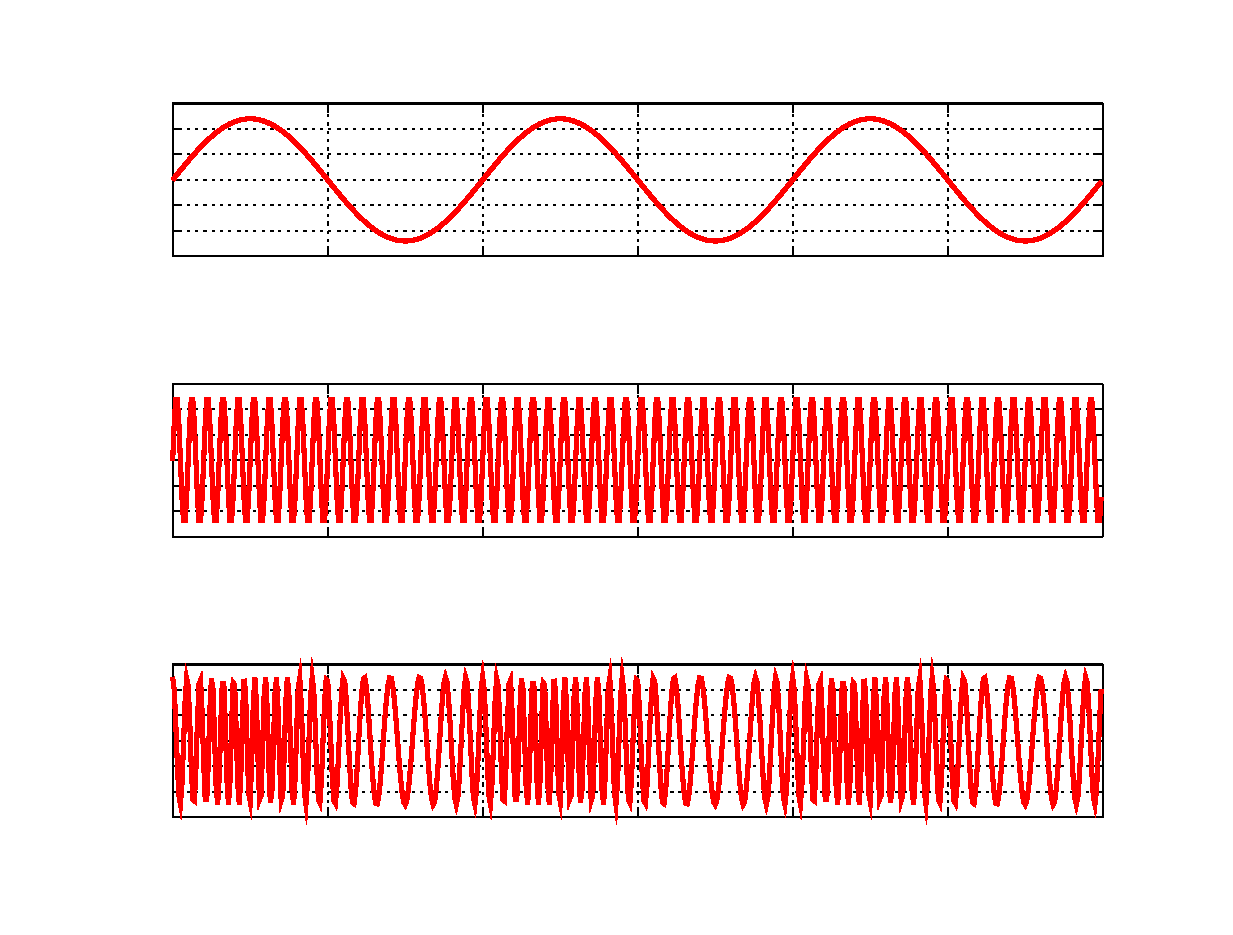
\includegraphics{fm-inc}
\end{picture}%
\begin{picture}(576,433)(0,0)
\fontsize{10}{0}
\selectfont\put(74.88,312.778){\makebox(0,0)[t]{\textcolor[rgb]{0,0,0}{{0}}}}
\fontsize{10}{0}
\selectfont\put(149.28,312.778){\makebox(0,0)[t]{\textcolor[rgb]{0,0,0}{{0.01}}}}
\fontsize{10}{0}
\selectfont\put(223.68,312.778){\makebox(0,0)[t]{\textcolor[rgb]{0,0,0}{{0.02}}}}
\fontsize{10}{0}
\selectfont\put(298.08,312.778){\makebox(0,0)[t]{\textcolor[rgb]{0,0,0}{{0.03}}}}
\fontsize{10}{0}
\selectfont\put(372.48,312.778){\makebox(0,0)[t]{\textcolor[rgb]{0,0,0}{{0.04}}}}
\fontsize{10}{0}
\selectfont\put(446.88,312.778){\makebox(0,0)[t]{\textcolor[rgb]{0,0,0}{{0.05}}}}
\fontsize{10}{0}
\selectfont\put(521.28,312.778){\makebox(0,0)[t]{\textcolor[rgb]{0,0,0}{{0.06}}}}
\fontsize{10}{0}
\selectfont\put(69.8755,317.799){\makebox(0,0)[r]{\textcolor[rgb]{0,0,0}{{-15}}}}
\fontsize{10}{0}
\selectfont\put(69.8755,330.02){\makebox(0,0)[r]{\textcolor[rgb]{0,0,0}{{-10}}}}
\fontsize{10}{0}
\selectfont\put(69.8755,342.24){\makebox(0,0)[r]{\textcolor[rgb]{0,0,0}{{-5}}}}
\fontsize{10}{0}
\selectfont\put(69.8755,354.46){\makebox(0,0)[r]{\textcolor[rgb]{0,0,0}{{0}}}}
\fontsize{10}{0}
\selectfont\put(69.8755,366.68){\makebox(0,0)[r]{\textcolor[rgb]{0,0,0}{{5}}}}
\fontsize{10}{0}
\selectfont\put(69.8755,378.9){\makebox(0,0)[r]{\textcolor[rgb]{0,0,0}{{10}}}}
\fontsize{10}{0}
\selectfont\put(69.8755,391.12){\makebox(0,0)[r]{\textcolor[rgb]{0,0,0}{{15}}}}
\fontsize{10}{0}
\selectfont\put(298.08,301.778){\makebox(0,0)[t]{\textcolor[rgb]{0,0,0}{{\frac{t}{s}}}}}
\fontsize{10}{0}
\selectfont\put(74.88,178.138){\makebox(0,0)[t]{\textcolor[rgb]{0,0,0}{{0}}}}
\fontsize{10}{0}
\selectfont\put(149.28,178.138){\makebox(0,0)[t]{\textcolor[rgb]{0,0,0}{{0.01}}}}
\fontsize{10}{0}
\selectfont\put(223.68,178.138){\makebox(0,0)[t]{\textcolor[rgb]{0,0,0}{{0.02}}}}
\fontsize{10}{0}
\selectfont\put(298.08,178.138){\makebox(0,0)[t]{\textcolor[rgb]{0,0,0}{{0.03}}}}
\fontsize{10}{0}
\selectfont\put(372.48,178.138){\makebox(0,0)[t]{\textcolor[rgb]{0,0,0}{{0.04}}}}
\fontsize{10}{0}
\selectfont\put(446.88,178.138){\makebox(0,0)[t]{\textcolor[rgb]{0,0,0}{{0.05}}}}
\fontsize{10}{0}
\selectfont\put(521.28,178.138){\makebox(0,0)[t]{\textcolor[rgb]{0,0,0}{{0.06}}}}
\fontsize{10}{0}
\selectfont\put(69.8755,183.16){\makebox(0,0)[r]{\textcolor[rgb]{0,0,0}{{-6}}}}
\fontsize{10}{0}
\selectfont\put(69.8755,195.38){\makebox(0,0)[r]{\textcolor[rgb]{0,0,0}{{-4}}}}
\fontsize{10}{0}
\selectfont\put(69.8755,207.6){\makebox(0,0)[r]{\textcolor[rgb]{0,0,0}{{-2}}}}
\fontsize{10}{0}
\selectfont\put(69.8755,219.82){\makebox(0,0)[r]{\textcolor[rgb]{0,0,0}{{0}}}}
\fontsize{10}{0}
\selectfont\put(69.8755,232.04){\makebox(0,0)[r]{\textcolor[rgb]{0,0,0}{{2}}}}
\fontsize{10}{0}
\selectfont\put(69.8755,244.26){\makebox(0,0)[r]{\textcolor[rgb]{0,0,0}{{4}}}}
\fontsize{10}{0}
\selectfont\put(69.8755,256.48){\makebox(0,0)[r]{\textcolor[rgb]{0,0,0}{{6}}}}
\fontsize{10}{0}
\selectfont\put(298.08,167.138){\makebox(0,0)[t]{\textcolor[rgb]{0,0,0}{{\frac{t}{s}}}}}
\fontsize{10}{0}
\selectfont\put(74.88,43.498){\makebox(0,0)[t]{\textcolor[rgb]{0,0,0}{{0}}}}
\fontsize{10}{0}
\selectfont\put(149.28,43.498){\makebox(0,0)[t]{\textcolor[rgb]{0,0,0}{{0.01}}}}
\fontsize{10}{0}
\selectfont\put(223.68,43.498){\makebox(0,0)[t]{\textcolor[rgb]{0,0,0}{{0.02}}}}
\fontsize{10}{0}
\selectfont\put(298.08,43.498){\makebox(0,0)[t]{\textcolor[rgb]{0,0,0}{{0.03}}}}
\fontsize{10}{0}
\selectfont\put(372.48,43.498){\makebox(0,0)[t]{\textcolor[rgb]{0,0,0}{{0.04}}}}
\fontsize{10}{0}
\selectfont\put(446.88,43.498){\makebox(0,0)[t]{\textcolor[rgb]{0,0,0}{{0.05}}}}
\fontsize{10}{0}
\selectfont\put(521.28,43.498){\makebox(0,0)[t]{\textcolor[rgb]{0,0,0}{{0.06}}}}
\fontsize{10}{0}
\selectfont\put(69.8755,48.52){\makebox(0,0)[r]{\textcolor[rgb]{0,0,0}{{-6}}}}
\fontsize{10}{0}
\selectfont\put(69.8755,60.74){\makebox(0,0)[r]{\textcolor[rgb]{0,0,0}{{-4}}}}
\fontsize{10}{0}
\selectfont\put(69.8755,72.96){\makebox(0,0)[r]{\textcolor[rgb]{0,0,0}{{-2}}}}
\fontsize{10}{0}
\selectfont\put(69.8755,85.18){\makebox(0,0)[r]{\textcolor[rgb]{0,0,0}{{0}}}}
\fontsize{10}{0}
\selectfont\put(69.8755,97.4001){\makebox(0,0)[r]{\textcolor[rgb]{0,0,0}{{2}}}}
\fontsize{10}{0}
\selectfont\put(69.8755,109.62){\makebox(0,0)[r]{\textcolor[rgb]{0,0,0}{{4}}}}
\fontsize{10}{0}
\selectfont\put(69.8755,121.84){\makebox(0,0)[r]{\textcolor[rgb]{0,0,0}{{6}}}}
\fontsize{10}{0}
\selectfont\put(298.08,32.4981){\makebox(0,0)[t]{\textcolor[rgb]{0,0,0}{{\frac{t}{s}}}}}
\fontsize{10}{0}
\selectfont\put(298.08,401.12){\makebox(0,0)[b]{\textcolor[rgb]{0,0,0}{{Nachrichtensignal}}}}
\fontsize{10}{0}
\selectfont\put(298.08,266.48){\makebox(0,0)[b]{\textcolor[rgb]{0,0,0}{{Trägersignal}}}}
\fontsize{10}{0}
\selectfont\put(298.08,131.84){\makebox(0,0)[b]{\textcolor[rgb]{0,0,0}{{Frequenzmodulieres Signal}}}}
\end{picture}
$\end{large}}
  \caption{Frequenzmodulation}
  \label{fig:fm}
\end{figure}
Die Frequenzmodulation verändert die Frequenz des Trägersignals linear zur Amplitude des Nachrichtensignals.
Eine Implementierung einer solchen Modulation ist mit einem Voltage contolled oscillator(VCO) simpel zu realisieren. Die Demodulation erfolgt über einen Diskriminator, welcher auf vielfältige Art und Weise aufgebaut werden kann. Exemplarisch sei an dieser Stelle die Demodulation mit einem Phase locked loop(PLL) genannt. Eine PLL führt die Ausgangsfrequenz immer einer gegeben Eingangsfrequenz nach. Die Regeldifferenz aus diesen Größen lässt sich als Spannung abgreifen. Wird ein frequenzmoduliertes Signal als Soll-Signal vorgegeben so ist die genannte Regelspannung das demodulierte Nachrichtensignal.

\subsubsection{Amplitudenmodulation}
\begin{figure}[H]
\centering
  \scalebox{0.7}{\begin{large}$\input{am.tex}$\end{large}}
  \caption{Amplitudenmodulation}
  \label{fig:am}
\end{figure}
Die Amplitudenmodulation verändert die Amplitude des Trägersignals proportional zum Nachrichtensignal.
Eine Amplitudenmodulation lässt sich durch Anwendung eines 4 Quadranten-Mischers unkompliziert implementieren. Zur Modulation werden lediglich ein Trägersignal, welches eine vielfache Frequenz des Nachrichtensignals haben muss, und das Nachrichtensignal multiplizert. Anschließend werden unerwünsche Mischprodukte herausgefiltert. Die Demodulation erfolgt über einen Tiefpass, dessen Grenzfrequenz weit unter der gewählten Trägerfrequenz liegt.
Da bei dieser Modulation die Information genauso wie bei der direkten Übertragung in der Amplitude liegt, entstehen wieder die gleichen Probleme durch die Dämpfung des Lichtwellenleiters.

\subsection{Digitale Übertragungsarten}
\subsubsection{Pulsweitenmodulation}
\begin{figure}[H]
\centering
  \scalebox{0.7}{\begin{large}
  $% GNUPLOT: LaTeX picture with Postscript
\begingroup
  \makeatletter
  \providecommand\color[2][]{%
    \GenericError{(gnuplot) \space\space\space\@spaces}{%
      Package color not loaded in conjunction with
      terminal option `colourtext'%
    }{See the gnuplot documentation for explanation.%
    }{Either use 'blacktext' in gnuplot or load the package
      color.sty in LaTeX.}%
    \renewcommand\color[2][]{}%
  }%
  \providecommand\includegraphics[2][]{%
    \GenericError{(gnuplot) \space\space\space\@spaces}{%
      Package graphicx or graphics not loaded%
    }{See the gnuplot documentation for explanation.%
    }{The gnuplot epslatex terminal needs graphicx.sty or graphics.sty.}%
    \renewcommand\includegraphics[2][]{}%
  }%
  \providecommand\rotatebox[2]{#2}%
  \@ifundefined{ifGPcolor}{%
    \newif\ifGPcolor
    \GPcolorfalse
  }{}%
  \@ifundefined{ifGPblacktext}{%
    \newif\ifGPblacktext
    \GPblacktexttrue
  }{}%
  % define a \g@addto@macro without @ in the name:
  \let\gplgaddtomacro\g@addto@macro
  % define empty templates for all commands taking text:
  \gdef\gplbacktext{}%
  \gdef\gplfronttext{}%
  \makeatother
  \ifGPblacktext
    % no textcolor at all
    \def\colorrgb#1{}%
    \def\colorgray#1{}%
  \else
    % gray or color?
    \ifGPcolor
      \def\colorrgb#1{\color[rgb]{#1}}%
      \def\colorgray#1{\color[gray]{#1}}%
      \expandafter\def\csname LTw\endcsname{\color{white}}%
      \expandafter\def\csname LTb\endcsname{\color{black}}%
      \expandafter\def\csname LTa\endcsname{\color{black}}%
      \expandafter\def\csname LT0\endcsname{\color[rgb]{1,0,0}}%
      \expandafter\def\csname LT1\endcsname{\color[rgb]{0,1,0}}%
      \expandafter\def\csname LT2\endcsname{\color[rgb]{0,0,1}}%
      \expandafter\def\csname LT3\endcsname{\color[rgb]{1,0,1}}%
      \expandafter\def\csname LT4\endcsname{\color[rgb]{0,1,1}}%
      \expandafter\def\csname LT5\endcsname{\color[rgb]{1,1,0}}%
      \expandafter\def\csname LT6\endcsname{\color[rgb]{0,0,0}}%
      \expandafter\def\csname LT7\endcsname{\color[rgb]{1,0.3,0}}%
      \expandafter\def\csname LT8\endcsname{\color[rgb]{0.5,0.5,0.5}}%
    \else
      % gray
      \def\colorrgb#1{\color{black}}%
      \def\colorgray#1{\color[gray]{#1}}%
      \expandafter\def\csname LTw\endcsname{\color{white}}%
      \expandafter\def\csname LTb\endcsname{\color{black}}%
      \expandafter\def\csname LTa\endcsname{\color{black}}%
      \expandafter\def\csname LT0\endcsname{\color{black}}%
      \expandafter\def\csname LT1\endcsname{\color{black}}%
      \expandafter\def\csname LT2\endcsname{\color{black}}%
      \expandafter\def\csname LT3\endcsname{\color{black}}%
      \expandafter\def\csname LT4\endcsname{\color{black}}%
      \expandafter\def\csname LT5\endcsname{\color{black}}%
      \expandafter\def\csname LT6\endcsname{\color{black}}%
      \expandafter\def\csname LT7\endcsname{\color{black}}%
      \expandafter\def\csname LT8\endcsname{\color{black}}%
    \fi
  \fi
    \setlength{\unitlength}{0.0500bp}%
    \ifx\gptboxheight\undefined%
      \newlength{\gptboxheight}%
      \newlength{\gptboxwidth}%
      \newsavebox{\gptboxtext}%
    \fi%
    \setlength{\fboxrule}{0.5pt}%
    \setlength{\fboxsep}{1pt}%
\begin{picture}(11520.00,8640.00)%
    \gplgaddtomacro\gplbacktext{%
      \colorrgb{0.00,0.00,0.00}%
      \put(1377,6335){\makebox(0,0)[r]{\strut{}-15}}%
      \colorrgb{0.00,0.00,0.00}%
      \put(1377,6611){\makebox(0,0)[r]{\strut{}-10}}%
      \colorrgb{0.00,0.00,0.00}%
      \put(1377,6887){\makebox(0,0)[r]{\strut{}-5}}%
      \colorrgb{0.00,0.00,0.00}%
      \put(1377,7163){\makebox(0,0)[r]{\strut{}0}}%
      \colorrgb{0.00,0.00,0.00}%
      \put(1377,7439){\makebox(0,0)[r]{\strut{}5}}%
      \colorrgb{0.00,0.00,0.00}%
      \put(1377,7715){\makebox(0,0)[r]{\strut{}10}}%
      \colorrgb{0.00,0.00,0.00}%
      \put(1377,7991){\makebox(0,0)[r]{\strut{}15}}%
      \colorrgb{0.00,0.00,0.00}%
      \put(1497,6135){\makebox(0,0){\strut{}0}}%
      \colorrgb{0.00,0.00,0.00}%
      \put(2985,6135){\makebox(0,0){\strut{}0.01}}%
      \colorrgb{0.00,0.00,0.00}%
      \put(4473,6135){\makebox(0,0){\strut{}0.02}}%
      \colorrgb{0.00,0.00,0.00}%
      \put(5961,6135){\makebox(0,0){\strut{}0.03}}%
      \colorrgb{0.00,0.00,0.00}%
      \put(7448,6135){\makebox(0,0){\strut{}0.04}}%
      \colorrgb{0.00,0.00,0.00}%
      \put(8936,6135){\makebox(0,0){\strut{}0.05}}%
      \colorrgb{0.00,0.00,0.00}%
      \put(10424,6135){\makebox(0,0){\strut{}0.06}}%
    }%
    \gplgaddtomacro\gplfronttext{%
      \colorrgb{0.00,0.00,0.00}%
      \put(797,7163){\rotatebox{90}{\makebox(0,0){\strut{}u_m/V}}}%
      \colorrgb{0.00,0.00,0.00}%
      \put(5960,5835){\makebox(0,0){\strut{}t/s}}%
      \colorrgb{0.00,0.00,0.00}%
      \put(5960,8191){\makebox(0,0){\strut{}Nachrichtensignal}}%
    }%
    \gplgaddtomacro\gplbacktext{%
      \colorrgb{0.00,0.00,0.00}%
      \put(1377,3643){\makebox(0,0)[r]{\strut{}-15}}%
      \colorrgb{0.00,0.00,0.00}%
      \put(1377,3919){\makebox(0,0)[r]{\strut{}-10}}%
      \colorrgb{0.00,0.00,0.00}%
      \put(1377,4195){\makebox(0,0)[r]{\strut{}-5}}%
      \colorrgb{0.00,0.00,0.00}%
      \put(1377,4471){\makebox(0,0)[r]{\strut{}0}}%
      \colorrgb{0.00,0.00,0.00}%
      \put(1377,4746){\makebox(0,0)[r]{\strut{}5}}%
      \colorrgb{0.00,0.00,0.00}%
      \put(1377,5022){\makebox(0,0)[r]{\strut{}10}}%
      \colorrgb{0.00,0.00,0.00}%
      \put(1377,5298){\makebox(0,0)[r]{\strut{}15}}%
      \colorrgb{0.00,0.00,0.00}%
      \put(1497,3443){\makebox(0,0){\strut{}0}}%
      \colorrgb{0.00,0.00,0.00}%
      \put(2985,3443){\makebox(0,0){\strut{}0.01}}%
      \colorrgb{0.00,0.00,0.00}%
      \put(4473,3443){\makebox(0,0){\strut{}0.02}}%
      \colorrgb{0.00,0.00,0.00}%
      \put(5961,3443){\makebox(0,0){\strut{}0.03}}%
      \colorrgb{0.00,0.00,0.00}%
      \put(7448,3443){\makebox(0,0){\strut{}0.04}}%
      \colorrgb{0.00,0.00,0.00}%
      \put(8936,3443){\makebox(0,0){\strut{}0.05}}%
      \colorrgb{0.00,0.00,0.00}%
      \put(10424,3443){\makebox(0,0){\strut{}0.06}}%
    }%
    \gplgaddtomacro\gplfronttext{%
      \colorrgb{0.00,0.00,0.00}%
      \put(797,4470){\rotatebox{90}{\makebox(0,0){\strut{}u_c/V}}}%
      \colorrgb{0.00,0.00,0.00}%
      \put(5960,3143){\makebox(0,0){\strut{}t/s}}%
      \colorrgb{0.00,0.00,0.00}%
      \put(5960,5498){\makebox(0,0){\strut{}Trägersignal}}%
    }%
    \gplgaddtomacro\gplbacktext{%
      \colorrgb{0.00,0.00,0.00}%
      \put(1377,950){\makebox(0,0)[r]{\strut{}-0.5}}%
      \colorrgb{0.00,0.00,0.00}%
      \put(1377,1344){\makebox(0,0)[r]{\strut{}0}}%
      \colorrgb{0.00,0.00,0.00}%
      \put(1377,1739){\makebox(0,0)[r]{\strut{}0.5}}%
      \colorrgb{0.00,0.00,0.00}%
      \put(1377,2133){\makebox(0,0)[r]{\strut{}1}}%
      \colorrgb{0.00,0.00,0.00}%
      \put(1377,2527){\makebox(0,0)[r]{\strut{}1.5}}%
      \colorrgb{0.00,0.00,0.00}%
      \put(1497,750){\makebox(0,0){\strut{}0}}%
      \colorrgb{0.00,0.00,0.00}%
      \put(2985,750){\makebox(0,0){\strut{}0.01}}%
      \colorrgb{0.00,0.00,0.00}%
      \put(4473,750){\makebox(0,0){\strut{}0.02}}%
      \colorrgb{0.00,0.00,0.00}%
      \put(5961,750){\makebox(0,0){\strut{}0.03}}%
      \colorrgb{0.00,0.00,0.00}%
      \put(7448,750){\makebox(0,0){\strut{}0.04}}%
      \colorrgb{0.00,0.00,0.00}%
      \put(8936,750){\makebox(0,0){\strut{}0.05}}%
      \colorrgb{0.00,0.00,0.00}%
      \put(10424,750){\makebox(0,0){\strut{}0.06}}%
    }%
    \gplgaddtomacro\gplfronttext{%
      \colorrgb{0.00,0.00,0.00}%
      \put(677,1778){\rotatebox{90}{\makebox(0,0){\strut{}u_{pwm}/V}}}%
      \colorrgb{0.00,0.00,0.00}%
      \put(5960,450){\makebox(0,0){\strut{}t/s}}%
      \colorrgb{0.00,0.00,0.00}%
      \put(5960,2806){\makebox(0,0){\strut{}Pulsweitenmoduliertes Signal}}%
    }%
    \gplbacktext
    \put(0,0){\includegraphics{pwm}}%
    \gplfronttext
  \end{picture}%
\endgroup
$
  \end{large}}
  \caption{Pulsweitenmodulation}
  \label{fig:pwm}
\end{figure}
Die Pulsweitenmodulation moduliert, ähnlich wie die Frequenzmodulation, das Nachrichtensignal im Zeitbereich. 
Die essentiellen Unterschiede liegen zum Einen darin, dass die PWM ein digitales Übertragungsverfahren ist und demnach nur 2 Zustände kennt, und zum Anderen, dass das Nachrichtensignal nicht direkt in der Frequenz des Trägersignals kodiert wird sondern in der Pulsweite des Trägersignals. Die Synthese einer Pulsweitenmodulation kann durch den Vergleich des Nachrichtensignals mit einer Dreiecksspannung erfolgen. Hierbei ist darauf zu achten, dass die Dreieckspannung, welche als Träger verwendet wird, eine vielfache Frequenz des Nachrichtensignals aufweist.Die Demodulation eines pulsweitenmodulierten Signals erfolgt durch einen Tiefpass, welcher ledglich das Nachrichtensignal im Passband hat. 




\subsection{Wahl des Übertragungsverfahren}
Eine unmodulierte Übertragung ist aufgrund der Leitungsdämpfung ausgeschlossen. Entsprechend kommt folgender genereller Systemaufbau in Frage.
\begin{figure}[H]
\centering
  \input{prinzip.pdf_tex}
  \caption{Prinzipieller Systemaufbau}
  \label{fig:psystem}
\end{figure}
Die Evaluation der 3 verbliebenen Varianten liefert die Pulsweitenmodulation(PWM) als optimales Ergebnis:
Im Gegensatz zu allen analogen Übertragungsverfahren lässt sich die PWM durch Übersteuerung des Eingangsverstärkers der Empfängereinheit sehr einfach rekonstruieren und ist demnach unempfindlich gegenüber Variationen der Dämpfung der Leitungslänge. Darüber hinaus ist die Synthese sowie Demodulation einer PWM mit einfachen Mitteln umzusetzen.\\
Neben den grundlegenden Aufgaben des Systems, wie Modulation und Demodulation, müssen noch weitere Komponenten wie eine Endstufe und eine Schutzschaltung gegenüber der Hochspannung im System verbaut werden. 
Aus allen vorangegangen Überlegungen geht folgender Systemaufbau hervor: 
\begin{figure}[H]
  \centering
  \input{systemaufbau.pdf_tex}
  \caption{Systemaufbau}
  \label{fig:system}
\end{figure}

\subsection{Pulsweitenmodulation - Theorie}
Im wesentlichen basiert die Funktionsweise einer PWM auf der Variation des Tastverhältnisses einer Rechteckspannung. Durch die Änderung des Tastverhältnis wird der Effektivwert der Rechteckspannung verändert, dieser berechnet sich wie folgt:\\
\begin{equation}
 U_{eff} = \sqrt{\frac{1}{T}\cdot\int\limits_{0}^T u(t)^2 dt}
\end{equation}
Offensichtlich ist der Effektivwert von dem Integral der Kurve über eine Periode, also der Fläche unter der Kurve, abhängig. Diese Fläche wird wie bereits beschrieben über das Tastverhältnis bestimmt. So kann jede Perdiode des Rechteckssignals als ein Abstastwert des Nachrichtensignals interpretiert werden. Dieses Integral ist beispielhaft für 2 Perioden eines Sinussignals in Abbildung \ref{fig:pwmArea} dargestellt. Aufgrund dieser Abtastung ist es wichtig, dass zur optimalen Rekonstruktion das 50 Hz Eingangssignal um ein Vielfaches abgetastet wird. Für diese Anwendung wurde eine 200-fache Überabtastung von $f_A=10kHz$ gewählt.
\begin{figure}[H]
  \centering
   \scalebox{0.6}{\begin{Large}
   \input{pwmArea.tex}
   \end{Large}}
   \caption{Pulsweitenmodulation Illustration}
  \label{fig:pwmArea}
\end{figure}

\newpage
